\subsection{Matched-power thermal comparison with translated ceramics}
The preceding subsection describes the geometry checkpoint; the following results extend it. Two newly solved conditional package cases compare the source 0.50 mm legs with the separately constructed 0.60 mm assembly at 300 K reservoir, 100 Pa krypton and 2 mW imposed die heat. Terminal current is solved as an unknown subject to $IV=0.595668$ W. The 88 individual nonlinear P/N legs couple to four source TET4 ceramic plates, whose geometry and 95 mapped source-face patches are rigidly translated with the assembly. Copper is a reduced multiport and the cavity is a reduced exchange model, not a full metal or gas field.

A geometry-derived interstage gas sensitivity uses three conservative parallel links,
\[
 A_j=W_{j+1}^{2}-n_j A_{\ell},\qquad G_j=\frac{k_g A_j}{d_j+2b_j},\qquad Q_j=G_j(T_{h,j}-T_{c,j}),
\]
where $A_{\ell}$ is the leg footprint, $d_j$ is the gap after the two metal films, and $b_j$ is the temperature-jump length. The areas are 17.76, 10.92 and 4.48 mm$^2$; $d_j$ is 0.57 mm or 0.67 mm for the two designs. Equal and opposite gas heat is applied to the adjacent ceramic plates. This is an engineering parallel-path proxy, not a solution of the connected interleg void.

\begin{center}\small\begin{tabular}{lrr}\toprule
Quantity & 0.50 mm & 0.60 mm \\ \midrule
Current (A) & 0.400298 & 0.370631 \\
Terminal voltage (V) & 1.488062 & 1.607175 \\
Terminal power (W) & 0.595668 & 0.595668 \\
Hot ceramic (K) & 303.761291 & 303.764120 \\
Top ceramic (K) & 219.297688 & 215.591806 \\
Die mount (K) & 219.368939 & 215.663617 \\
Cold P/N leg $Q_c$, before parasitics (mW) & 6.099 & 6.051 \\
Sink rejection (W) & 0.592285 & 0.592474 \\
\bottomrule\end{tabular}\end{center}

The custom case is 3.705 K colder at the mount under these particular assumptions. It is not a measured cooling improvement or a global optimum. The fixed external 3 mm gas-to-reservoir proxy and gray view factors are unchanged; their volume may overlap the new interstage approximation. At the archived fixed temperature field, changing only the external proxy gap from 1.5 to 3 to 6 mm gives 6.319, 3.420 and 1.783 mW of external gas heating, respectively; this is a fixed-field sensitivity, not a coupled uncertainty bound.

\begin{figure}[htbp]\centering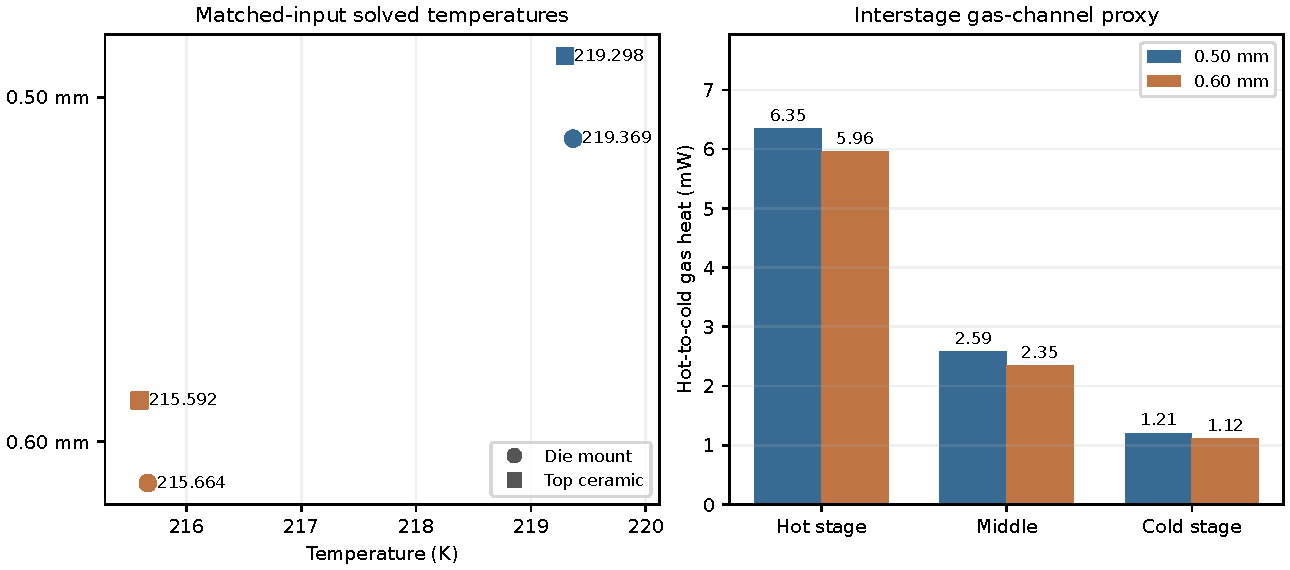
\includegraphics[width=.96\linewidth]{figures/v320_height_matched.pdf}\caption{Actual coupled-solver outputs at matched electrical input. Left: solved die and upper-ceramic temperatures; right: calculated interstage gas heat from warmer to colder plates. The external gas and radiation paths and the reduced metal network are conditional proxies.}\end{figure}

The source Cu return paths and detector bond lengths are recalculated for the candidate. The middle return foot remains a thermal port; its previously counted electrical series contact is excluded in both cases. Independent reconstruction checks each leg, all stage boundaries, copper and lead Joule heat, gas, die and sink. The largest stage-boundary and global residuals are $1.21\times10^{-9}$ W and $1.05\times10^{-9}$ W; maximum leg residual is $1.48\times10^{-13}$ W. Final spatial updates are below $2.0\times10^{-7}$ K. The source research specimens are unmatched, and temperatures above 300 K use an assumed continuation. The old 3D electrical-contact and raw-flux failures remain unchanged.
